\documentclass[12pt, letter]{article}

\usepackage[margin=1in, ignorefoot]{geometry} 
\usepackage[english]{babel}
\usepackage{amsmath, amssymb, amsthm, amsfonts}
\usepackage[usenames,dvipsnames]{xcolor}
\usepackage{ucs}
\usepackage{tabularx}
\usepackage{graphicx}
\usepackage{booktabs}
\usepackage{multirow}
\usepackage{subscript}
\usepackage{setspace}
\usepackage{ccicons}
\usepackage{txfonts}
\usepackage{fontawesome}
\usepackage{hologo}

\usepackage{natbib}
\bibpunct{(}{)}{;}{a}{}{,}
\bibliographystyle{apsr}
\usepackage[nottoc,notlot,notlof,numbib]{tocbibind}
\def\fns{\footnotesize}

\setlength\parindent{0pt}

\definecolor{cerulean}{rgb}{0.0, 0.48, 0.65}
\definecolor{pansypurple}{rgb}{0.47, 0.09, 0.29}

\DeclareMathOperator{\var}{var}

\usepackage[bookmarks, colorlinks, breaklinks]{hyperref}  
\hypersetup{
	linkcolor=black,
	citecolor=cerulean,
	filecolor=black,
	urlcolor=pansypurple,
	pdftitle={Brief Introduction to R}, 
    pdfauthor={Anna Walsdorff}
} 

\usepackage{chngcntr}
\renewcommand{\thesection}{\Roman{section}}
\counterwithout{subsection}{section}

% listings

\usepackage{listings, color}
\definecolor{mygreen}{rgb}{0,0.6,0}
\definecolor{mygray}{rgb}{0.5,0.5,0.5}
\definecolor{mymauve}{rgb}{0.58,0,0.82}
\definecolor{light-gray}{gray}{0.98}
\definecolor{lighteccru}{HTML}{F6F4EE}
\usepackage{courier}
%%
\lstset{ %
  backgroundcolor=\color{lighteccru},   % choose the background color; you must add \usepackage{color} or \usepackage{xcolor}
  basicstyle=\footnotesize\ttfamily,        % the size of the fonts that are used for the code
  breaklines=true,                 % sets automatic line breaking
  captionpos=b,                    % sets the caption-position to bottom
  commentstyle=\color{mygreen},    % comment style
  keywordstyle=\color{blue},       % keyword style
  language={R},               	   % the language of the code
  numbers=none,                    % where to put the line-numbers; possible values are (none, left, right)
  numbersep=5pt,                   % how far the line-numbers are from the code
  numberstyle=\tiny\color{mygray}, % the style that is used for the line-numbers
  rulecolor=\color{black},         % if not set, the frame-color may be changed on line-breaks within not-black text (e.g. comments (green here))
  showspaces=false,                % show spaces everywhere adding particular underscores; it overrides 'showstringspaces'
  showstringspaces=false,          % underline spaces within strings only
  showtabs=false,                  % show tabs within strings adding particular underscores                    % sets default tabsize to 2 spaces
  title=\lstname,                   % show the filename of files included with \lstinputlisting; also try caption instead of title
  belowskip=0em,
  belowcaptionskip=0em 
}

\newcommand{\R}{\textsf{R}\ }

% Font

\usepackage{fontspec}
\defaultfontfeatures{Mapping=tex-text}
\setsansfont[Scale=MatchLowercase]{Helvetica Neue}
%\setsansfont{LeMondeSans:style=Regular}
\setmainfont[BoldFont = Garamond Premier Pro Semibold]{GaramondPremrPro-Med}

\usepackage[math]{mathspec}
\setmathfont(Digits,Latin,Greek){GaramondPremrPro-Med}
%\setmathfont{Latin Modern Math}[version=lm]

\renewcommand\ttdefault{lmtt}

\linespread{1.1}         

%\usepackage{tgadventor}     % this looks pretty awesome

%\usepackage{sectsty}
%\sectionfont{\fontsize{16}{15}\sffamily}
%\subsectionfont{\fontsize{14}{15}\sffamily}


\usepackage{enumitem}% http://ctan.org/pkg/enumitem
\newtheorem{cslist}{Hypothesis}
\renewcommand{\thecslist}{H\arabic{cslist}}%
\newtheorem{thm}{Theorem}
\newtheorem{claim}{Claim}
\newtheorem{proposition}{Proposition}
\newtheorem{lemma}{Lemma}

%\doublespacing
%\onehalfspacing
%\singlespacing
%\setlength{\parindent}{2ex}


\usepackage{titling}
\newcommand{\subtitle}[1]{%
  \posttitle{%
    \par\end{center}
    \begin{center}\large#1\end{center}
    \vskip0.5em}%
}

\title{Brief Introduction to \R}
\author{Prepared by Anna Walsdorff \\ \href{mailto:anna.walsdorff@rochester.edu}{\texttt{anna.walsdorff@rochester.edu}}}
\date{Updated: September 28, 2018}

% DOCUMENT
\begin{document}

\begin{titlepage}

\maketitle

\vspace*{4cm}
\thispagestyle{empty}

\end{titlepage}


\newpage

\section*{License}
\thispagestyle{empty}

\noindent%
This document is released under the Creative Commons Attribution license
(\ccby), {\small \url{http://creativecommons.org/licenses/by/3.0/}}.

\bigskip%
\noindent%
The source code for this document is available on Github at
{\small \url{https://github.com/ffrodslaw/r-intro}}.

\bigskip%
\noindent%
This document contains and incorporates material from notes by \href{https://drive.google.com/file/d/0BzD2LimxGIzIeWppdWxCZHR1T2M/view?usp=sharing}{Casey Crisman-Cox} and  \href{https://cran.r-project.org/doc/manuals/r-release/R-intro.pdf}{the R Core Team}.

\pagebreak

{\small \tableofcontents}
\thispagestyle{empty}

\pagebreak
\setcounter{page}{1}

\section{The basics of \R}
\subsubsection*{Advantages}

Why do we care?
\begin{itemize}
\item It's open source and free
\item It's available for all major platforms (Win, Mac, Linux)
\item Easy to find support online
\item Frequent updates
\item Very flexible 

\end{itemize}

\subsubsection*{Not so great}

\begin{itemize}
\item No graphical user interface (like Stata or SPSS)
\item You don't ``see'' what you're doing to the data (like Excel)
\item Can be difficult to learn
\item No warranty whatsoever
\end{itemize}

\subsection{Installing R}

Go to\ \ {\small \url{https://cran.r-project.org/}} and choose your operating system under ``Download and Install R''.

\subsubsection*{Windows}

Choose ``base" to get to the base distribution and then download the latest version. 

\subsubsection*{Mac}

Installing \R on your Mac should be pretty similar. Choose the version that matches your Mac. For example, if you run Mac OS X 10.11 or higher, download the ``R-3.5.1.pkg" package.

\subsubsection*{Linux}

Find your distribution and follow the instructions. This is a little less straightforward than with Windows and Mac but if you run into any trouble email me.


\subsubsection*{Installing an editor}

Once you have \R installed, you have full access to its functions. \R comes installed with a terminal that you use to send commands. While it works just fine, it is not the easiest to learn.

We will use an editor for ease of use and organization. \R Studio is an excellent alternative to the console as it provides a nice system to edit your files while you're working on them and keeps everything better organized.

To download \R Studio, visit\ \  {\small \url{https://www.rstudio.com/products/rstudio/download/#download}} and find the installer that matches your system.

\subsubsection*{How does it work?}

\R is a compiled language which means that it executes your code immediately (no need to build an entire program).

When you start \textsf{R}, you see information about the version, software licence etc. and the \emph{prompt}:

\begin{lstlisting}
>
\end{lstlisting}

This tells you that \R is waiting for you. Your typed command appears next to the prompt and can be executed by hitting \texttt{Enter}.

\subsection{\R as a calculator}

\begin{lstlisting}
> 1 + 2
[1] 3
\end{lstlisting}

By executing this command, \textsf{R} creates an \textit{object} and prints the content of the object. The \texttt{[1]} denotes that the object only has one value.

It can happen that you see a different prompt, a \texttt{+} instead of a \texttt{>}. This means that \textsf{R} is waiting for more input and the current command is not complete.

\begin{lstlisting}
> 1 +
+ 2
[1] 3
\end{lstlisting} 

A frequent problem are brackets, you might have opened one but didn't close it. \R doesn't know what to do and waits for further input. Give \R what it wants.

\begin{lstlisting}
> 7 / (1 + 3
+ )
[1] 1.75
\end{lstlisting}

(Note: this is not the same as \texttt{7 / 1 + 3} .)

\vspace*{0.5cm}

\newpage
\subsubsection*{Operators}

\textsf{R} understands these basic operators

\begin{itemize}
\item $+$ and $-$ for addition and subtraction
\item $*$ and $/$ for multiplication and division
\item $\wedge$ for exponents
\end{itemize}

Standard functions are also available:

\begin{lstlisting}
> log(10)     #base= e
[1] 2.302585

> log(10, base=10)
[1] 1

> exp(1)
[1] 2.718282

> sin(0)
[1] 0

> acos(-1)
[1] 3.141593
\end{lstlisting}

\textsf{R} can't do the impossible:

\begin{lstlisting}
> log(0)
[1] -Inf

> log(-1)
Warning in log(-1): NaNs produced
[1] NaN
\end{lstlisting}

Where \texttt{-Inf} means $-\infty$ and \texttt{NaN} means ``Not a Number''. Getting those is a sign that you need to stop and reevaluate what you're doing.

\subsubsection*{Comments and Spacing}

It is great to annotate your code. This will remind you or everyone else who reads your code of what you did. The command for that is \texttt{\#}; \texttt{R} ignores everything printed after it (until the line ends).

\begin{lstlisting}
> 1 + 2  # always annotate
[1] 3
\end{lstlisting}

\textsf{R} does not care about how many spaces you put in your commands.

\subsection{Vectors and objects}

Basically everything in \R is an object. \R creates and manipulates objects. Having information stored as objects allows you to call it later on. Examples of objects are integers, vectors, matrices, lists and data frames. In \R an assignment can take many forms, and all of the following are the same.

\begin{lstlisting}
> x <- exp(1)
> x = exp(1)
> exp(1) -> x
> assign('x', exp(1))
\end{lstlisting}

When you want to assign an object, you give it a name. Descriptive names can be useful when you have to handle many objects. Use \texttt{<-} or \texttt{=} to assign an object (most \R users prefer the former). Any name that does not start with a number is fine. Note that \texttt{R} is case-sensitive.

Once a value is assigned to the variable we can use \texttt{x} like any other number.

\begin{lstlisting}
> x
[1] 2.718282

> x-2
[1] 0.7182818

> log(x)
[1] 1
\end{lstlisting}

Notice that none of the above actually change the value of x. If we want to assign a new value to \texttt{x} we just use the arrow again.

\begin{lstlisting}
> x
[1] 2.718282

> x <- exp(2)

> x
[1] 7.389056
\end{lstlisting}


%\newpage
%\subsection*{R Code}
 % % % % % % % % % % % % THIS IS WHERE I ACTUALLY DO THE LISTINGS % % % % % % % % % % % %
%\lstinputlisting{01.R}

\subsubsection*{Vectors}
 
Notice that all of our output began with the symbol \texttt{[1]}, for example

\begin{lstlisting}
> 2+2

[1] 4
\end{lstlisting}

The just means that R thinks of this as a vector(a set of numbers) and the \texttt{[1]} tells you that the value next to it is the first number in the vector. There's no reason why an variable in \R has to have only one value. The simplest way to create vector is with the \texttt{c()} function.

\begin{lstlisting}
> x <- c(1, 4, 6, 1)

> x
[1] 1 4 6 1
\end{lstlisting}

The \texttt{[1]} is still there to tell us that the number next to it is the first value in the vector. The \texttt{c} in this function stands for ``concatenate'' and it can be used to bring lots of vectors together.

\begin{lstlisting}
> y <- c(2, 3, 2, 1)
> c(y, y, y, x, x, x, y, y, x, x)

[1] 2 3 2 1 2 3 2 1 2 3 2 1 1 4 6 1 1 4 6 1 1 4 6 1 2 3 2 1 2 3 2 1 1 4 6
[36] 1 1 4 6 1
\end{lstlisting}

Whenever the output goes onto a second line we get a new indicator to tell us what position it is. So in the code above we have \texttt{[1]} at the beginning of the output and then \texttt{[36]} which tells us that the value that starts the second line is the 36th value in the vector.

\vspace*{0.5cm}

Nearly all the functions we looked at before work on vectors.

\begin{lstlisting}
> x+y
[1] 3 7 8 2

> x/y
[1] 0.500000 1.333333 3.000000 1.000000

> log(x)
[1] 0.000000 1.386294 1.791759 0.000000
\end{lstlisting}

We can also sort the values within a vector.

\begin{lstlisting}
> sort(x)
[1] 1 1 4 6

> sort(x, decreasing=TRUE)
[1] 6 4 1 1

> length(x)
[1] 4
\end{lstlisting}

\subsubsection*{Easier ways to create vectors}

If we are creating a vector that follows a pattern, we do not have manually type out every element of it. For consecutive integers, we can use a colon.

\begin{lstlisting}
> 1:15
 [1]  1  2  3  4  5  6  7  8  9 10 11 12 13 14 15
 
> 5:2
[1] 5 4 3 2
\end{lstlisting}

The more general version of the colon is the \verb|seq()| command.

\begin{lstlisting}
> seq(0,20)
 [1]  0  1  2  3  4  5  6  7  8  9 10 11 12 13 14 15 16 17 18 19 20
 
> seq(0, 20, by = 2)
 [1]  0  2  4  6  8 10 12 14 16 18 20
 
> seq(0, 20, length.out = 5)
[1]  0  5 10 15 20
\end{lstlisting}

The \verb|rep()| command allows you to repeat numbers.

\begin{lstlisting}
> rep(10, 2)
[1] 10 10

> rep(x,3)
 [1] 1 4 6 1 1 4 6 1 1 4 6 1
 
> rep(x, each = 3)  # repeats each number within x one at a time
 [1] 1 1 1 4 4 4 6 6 6 1 1 1
\end{lstlisting}

Note here that a vector can also include non-numerical elements. For example,

\begin{lstlisting}
> animals <- c("cat", "beaver", "raccoon")
\end{lstlisting}

\subsubsection*{Indexing}

We use indexing when we want to extract or replace a single value within a vector. For this we use square brackets.

\begin{lstlisting}
> z <- seq(0, 6, by = 2)
> z[3]
[1] 4

> z[1:3]  # first three values
[1] 0 2 4

> z[c(1,3)]  # values 1 and 3, note that we need c()
[1] 0 4

> z[-c(1,3)]  # everything but values 1 and 3
[1] 2 6
\end{lstlisting}

We can also extract using logical operators. Assume we only want elements of \verb|z| that are greater than 4. 

\begin{lstlisting}
> z>4
[1] FALSE FALSE FALSE  TRUE
\end{lstlisting}

The command returns a vector of \texttt{TRUE} and \texttt{FALSE} values to show whether a certain element in \texttt{z} fulfills the condition. In order to get the elements that meet the conditions, we can subset the vector again.

\begin{lstlisting}
> z[z>4]
[1] 6
\end{lstlisting}

Commonly used logical operators are \verb|<| (less than), \verb|<=| (less than or equal to), \verb|>| (greater than), \verb|>=| (greater than or equal to), \verb|==| (equal), \verb|!=| (not equal), and \verb|!| (not). Logical operators can be strung together using \verb|&| (and) and \texttt{|} (or).

\begin{lstlisting}
> z > 3 & z < 5
[1] FALSE FALSE  TRUE FALSE

> z[z > 3 & z < 5]
[1] 4

> z[z > 3 | z < 5]
[1] 0 2 4 6
\end{lstlisting}

\subsubsection*{Removing objects}

We use the \verb|ls()| command to view all the objects that we have defined. 

\begin{lstlisting}
> ls()
[1] "animals" "x" "y" "z"
\end{lstlisting}

If we want to remove one of them, we can use the \verb|rm()| command. It cannot be undone, so be careful with it.

\begin{lstlisting}
> rm(list='z')
> ls()
[1] "animals" "x" "y"
\end{lstlisting}

We can also delete one than one object at a time by using the \verb|c()| command, for example \verb|rm(list = c('x', 'y'))|. The command \verb|rm(list=ls())| deletes everything.

\subsection{Matrices}

Matrices are two-dimensional versions of vectors. To create a matrix in \R, you just need to create a vector and tell \R the dimensions.

\begin{lstlisting}
> matrix(x, nrow = 2)
     [,1] [,2] [,3] [,4] [,5]
[1,]    1    3    5    7    9
[2,]    2    4    6    8   10

> matrix(x, ncol = 2)
     [,1] [,2]
[1,]    1    6
[2,]    2    7
[3,]    3    8
[4,]    4    9
[5,]    5   10
\end{lstlisting}

\R fills in the numbers column by column, but we can force it to do it by row:

\begin{lstlisting}
> matrix(x, ncol = 2, byrow = TRUE)
     [,1] [,2]
[1,]    1    2
[2,]    3    4
[3,]    5    6
[4,]    7    8
[5,]    9   10
\end{lstlisting}

We can also use \verb|cbind| and \verb|rbind| to ``bind'' vectors together to make a matrix, bind a vector to a matrix, or bind matrices together.

\begin{lstlisting}
> cbind(x, y)
       x   y
 [1,]  1 -10
 [2,]  2  -9
 [3,]  3  -8
 [4,]  4  -7
 [5,]  5  -6
 [6,]  6  -5
 [7,]  7  -4
 [8,]  8  -3
 [9,]  9  -2
[10,] 10  -1

> rbind(x, y)
  [,1] [,2] [,3] [,4] [,5] [,6] [,7] [,8] [,9] [,10]
x    1    2    3    4    5    6    7    8    9    10
y  -10   -9   -8   -7   -6   -5   -4   -3   -2    -1
\end{lstlisting}

Another useful command for matrices is \verb|diag()|. It has a few different uses.

\begin{lstlisting}
> diag(3)  # 3 x 3 identity matrix
     [,1] [,2] [,3]
[1,]    1    0    0
[2,]    0    1    0
[3,]    0    0    1

> diag(x)  # square matrix with diagonal = x, off-diagonal = 0
      [,1] [,2] [,3] [,4] [,5] [,6] [,7] [,8] [,9] [,10]
 [1,]    1    0    0    0    0    0    0    0    0     0
 [2,]    0    2    0    0    0    0    0    0    0     0
 [3,]    0    0    3    0    0    0    0    0    0     0
 [4,]    0    0    0    4    0    0    0    0    0     0
 [5,]    0    0    0    0    5    0    0    0    0     0
 [6,]    0    0    0    0    0    6    0    0    0     0
 [7,]    0    0    0    0    0    0    7    0    0     0
 [8,]    0    0    0    0    0    0    0    8    0     0
 [9,]    0    0    0    0    0    0    0    0    9     0
[10,]    0    0    0    0    0    0    0    0    0    10

> Z <- matrix(1:9, nrow = 3)
> Z
     [,1] [,2] [,3]
[1,]    1    4    7
[2,]    2    5    8
[3,]    3    6    9

> diag(Z)  # extract the diagonal of a square matrix
[1] 1 5 9
\end{lstlisting}

You can also turn a matrix back into a vector.

\begin{lstlisting}
> c(Z)
[1] 1 2 3 4 5 6 7 8 9

> as.vector(Z)
[1] 1 2 3 4 5 6 7 8 9
\end{lstlisting}

Any time you want to check what kind of object something is, you can check its class.

\begin{lstlisting}
> class(x)
[1] "integer"

> class(Z)
[1] "matrix"
\end{lstlisting}

\subsubsection*{Matrix attributes}

Just like with vectors we can use square brackets  to extract or replace elements. For a matrix \texttt{X}, the command \verb|X[i, j]| gives you the element from row \texttt{i}, column \texttt{j}.

\begin{lstlisting}
> X <- matrix(1:12, nrow = 3)
> X
     [,1] [,2] [,3] [,4]
[1,]    1    4    7   10
[2,]    2    5    8   11
[3,]    3    6    9   12
> X[2,4]
[1] 11

> X[3,2] <- 8
> X
     [,1] [,2] [,3] [,4]
[1,]    1    4    7   10
[2,]    2    5    8   11
[3,]    3    8    9   12

> X[1,]  # extracts the whole first row
[1]  1  4  7 10

> X[, 2]  # extracts the second column
[1] 4 5 8

> X[1:2,]  # first two rows
     [,1] [,2] [,3] [,4]
[1,]    1    4    7   10
[2,]    2    5    8   11
\end{lstlisting}

As before, we can use logical operators.

\begin{lstlisting}
> X[ ,2] == 8  # which rows have 8 in the second column?
[1] FALSE FALSE  TRUE

> X[X[ ,2] == 8, ]  # pulls out the corresponding elements
[1]  3  8  9 12
\end{lstlisting}

For most things, \R treats matrices as vectors that are written differently and we can do operations with it such as asking for their length, mean, standard deviation, etc.

\begin{lstlisting}
> length(X)
[1] 12

> mean(X)
[1] 6.666667

> sd(X)
[1] 3.626502
\end{lstlisting}

Commands that only work with matrices include:

\begin{lstlisting}
> dim(X)
[1] 3 4

> nrow(X)
[1] 3

> ncol(X)
[1] 4
\end{lstlisting}

Another thing that can be done with matrices but not with vectors is naming the rows and columns. Both of the names are just string vectors and can be set with, e.g. \verb|colnames(X) <- c("left", "right")| and \verb|rownames(X) <- c("up", "down")|.

\subsubsection*{Matrix operations}

Matrix math in \R includes standard operations including arithmetic.

\begin{lstlisting}
> X <- matrix(1:4, nrow = 2)
> Y <- diag(2)

> X + Y
     [,1] [,2]
[1,]    2    3
[2,]    2    5

> X-Y
     [,1] [,2]
[1,]    0    3
[2,]    2    3

> X * Y  # element-wise multiplication
     [,1] [,2]
[1,]    1    0
[2,]    0    4

> X %*% Y  # matrix multiplication
     [,1] [,2]
[1,]    1    3
[2,]    2    4
\end{lstlisting}

If you use matrix multiplication on a vector \R will guess whether it is a row or column vector. It might guess wrong occasionally, so be careful. We can also transpose and invert matrices.

\begin{lstlisting}
> X
     [,1] [,2]
[1,]    1    3
[2,]    2    4

> t(X)  # transpose
     [,1] [,2]
[1,]    1    2
[2,]    3    4

> solve(X)  # invert
     [,1] [,2]
[1,]   -2  1.5
[2,]    1 -0.5
\end{lstlisting}

Other handy function include the determinant of the Cholesky decomposition.

\begin{lstlisting}
> Y <- matrix(c(1, 0.5, 0.5, 1), nrow = 2)

> det(Y)
[1] 0.75

> chol(Y)  # Choleski decomposition
     [,1]      [,2]
[1,]    1 0.5000000
[2,]    0 0.8660254

> t(chol(Y)) %*% chol(Y) 
     [,1] [,2]
[1,]  1.0  0.5
[2,]  0.5  1.0
\end{lstlisting}

Other things that will be useful are the trace as well as eigenvalues and eigenvectors of matrices.

\begin{lstlisting}
> sum(diag(Y))  # there is no command for the trace
[1] 2

> eigen(Y)
eigen() decomposition
$values
[1] 1.5 0.5

$vectors
          [,1]       [,2]
[1,] 0.7071068 -0.7071068
[2,] 0.7071068  0.7071068
\end{lstlisting}

\subsection{Lists}

When \R returns a list to us, we can extract the elements of it using the dollar sign. The names are given by the output. In the \texttt{eigen()} example above the names are given as ``values'' and ``vectors''.

\begin{lstlisting}
> eigen(Y)$values
[1] 1.5 0.5

> eigen(Y)$vectors
          [,1]       [,2]
[1,] 0.7071068 -0.7071068
[2,] 0.7071068  0.7071068
\end{lstlisting}

Alternatively, we can still use brackets but we need to double them up when we are dealing with lists.

\begin{lstlisting}
> eigen(Y)[[2]]
          [,1]       [,2]
[1,] 0.7071068 -0.7071068
[2,] 0.7071068  0.7071068

> class(eigen(Y)[[2]])
[1] "matrix"
\end{lstlisting}

\subsection{Packages and updating}

Packages expand the functionality of \R. They are free and can be downloaded from CRAN (and to a much smaller extent from other sources). You can directly install them in the console. 

\begin{lstlisting}
> install.packages("MASS")
\end{lstlisting}

It may ask you to pick a mirror. Choose whichever you want. After the package it installed, you can load it.

\begin{lstlisting}
> library(MASS)
\end{lstlisting}

\subsubsection*{Updating \R and \R packages}

To update \R, you need to 1) download the new version, 2) install it, and 3) uninstall the old version. If there is a major upgrade, you may need to copy files from your library folder to the new once before uninstalling the old version. This save you from reinstalling all of your packages.

To update an \R package, simply run \verb|install.packages()| again or use RStudio's function for it in the ``Tools'' menu.

\subsection{Getting help}

You will likely run into a lot of problem. This is normal and happens even to the most senior \R users. One way to solve it is to look up the \R help file of the particular function that you are curious about.

\begin{lstlisting}
> ?log
> help(log)
\end{lstlisting}

Both commands do the same. The help file consists of multiple sections such as what the function is supposed to do, what arguments it takes, more details, and an example of its use. If you know what you want to do, but don't know what function to use, you can search for that as well:

\begin{lstlisting}
> ??"multivariate normal"
> help.search("multivariate normal")
\end{lstlisting}

If neither solves your problem, Google will nearly always find you the right answer, especially answers from \href{htpp://www.stackoverflow.com}{Stack Overflow}.






\newpage
\section{Programming}
\subsection{Control statements}

\subsubsection*{Conditional}

For logical conditions we can use \texttt{if} and \texttt{else} as separate commands.

\begin{lstlisting}
> if (logical){
  command1
  command2
}else{
  command3
}
\end{lstlisting}

A trivial example of an if else statement is

\begin{lstlisting}
> y <- FALSE
> if(y){
+   cat("Hello World")
+ }else{
+   cat("Goodbye")
+ }

Goodbye
\end{lstlisting}

There also is a vectorized version of the \texttt{if/else} construct, the \texttt{ifelse} function.

\begin{lstlisting}
ifelse(condition, a, b)
\end{lstlisting}

It returns \texttt{a} if the condition is fulfilled and \texttt{b} if not.

\subsubsection*{Repetitive}

A loop repeatedly goes over the same code for a list of different objects. The most basic form in \R is the \texttt{for} loop.

\begin{lstlisting}
> y <- 1:10
> for(i in 1:10){
+   y[i] <- y[i]^2
+ }
> y
 [1]   1   4   9  16  25  36  49  64  81 100
\end{lstlisting}

The \texttt{break} command is useful when you are repeating a process but do not care about how many times it is done, just that it is. For example, you want something to converge.

\begin{lstlisting}
> repeat{
+   y <- runif(1)
+   if(y < 0.05){
+     break
+   }
+ }
> y
[1] 0.02829025
\end{lstlisting}

Alternatively (and easier), you can use the \texttt{while} structure which basically functions like a \texttt{for} loop with a built-in stop command.

\begin{lstlisting}
> y <- 1
> while(y > 0.05){
+   y <- runif(1)
+ }
> y
[1] 0.02105261
\end{lstlisting}

\subsection{*ply functions}

The ply family is a set of functions with the goal of making code faster and more readable. They can often be used to avoid writing out lengthy loops. The most basic one of them, \texttt{apply}, is used on vectors.

\begin{lstlisting}
> X <- replicate(3, rnorm(10))
> apply(X, 2, sd)  # standard deviation of every column
[1] 0.9302021 1.3075942 0.9424055
\end{lstlisting}

The options \texttt{2} refers to column while \texttt{1} refers to rows.

\begin{lstlisting}
> apply(X, 1, max) 
 [1]  0.6140781  0.5996994  0.8903101  0.5666874  1.2870948
 [6]  2.1704159 -0.7683647 -0.3774086  0.5831079  1.0580204
\end{lstlisting}

When you're dealing with lists you can use \texttt{lapply}.

\begin{lstlisting}
> X <- list(A = diag(1:4),
+           B = matrix(1:4, nrow = 2))
> lapply(X, solve)
$A
     [,1] [,2]      [,3] [,4]
[1,]    1  0.0 0.0000000 0.00
[2,]    0  0.5 0.0000000 0.00
[3,]    0  0.0 0.3333333 0.00
[4,]    0  0.0 0.0000000 0.25

$B
     [,1] [,2]
[1,]   -2  1.5
[2,]    1 -0.5
\end{lstlisting}

If you want to do an operations on a list that returns a vector instead, you can use \texttt{sapply}.

\begin{lstlisting}
> X <- list(A = diag(1:4),
+           B = matrix(1:4, nrow = 2))
> sapply(X, max)
A B 
4 4 
\end{lstlisting}

\subsection{Write your own function} 

One of the great things about \R is that it allows you to write your own functions in a relatively simple and elegant way. Customizing \R by writing your own function will make your experience with it much easier and more comfortable. Most canned commands are written in \R itself. For example, check out the source code of the \texttt{rowMeans} command by typing the command without any parentheses into the console.

A function is defined in the form

\begin{lstlisting}
> name <- function(arg_1, arg_1, ...) expression
\end{lstlisting}

For example, you could write your own function that calculates the sum of squares.

\begin{lstlisting}
> sum_of_squares <- function(x, y) {
+   x^2 + y^2
+ }

< sum_of_squares(2,5)
29
\end{lstlisting}

\subsubsection*{Named arguments and defaults}

If argument to called functions are given in the ``\texttt{name = object}'' form, they can be given in any order. In the example above, the call \verb|sum_of_squares(y = 5, x = 2)| will yield the same result.

When writing your own function, you can specify default values of arguments. This means that they are not necessary to be included in the call. In the same example above, if we set \texttt{y}'s default to 10, we would not need to specify it every time.

\begin{lstlisting}
> sum_of_squares <- function(x, y = 10) {
+   x^2 + y^2
+ }

< sum_of_squares(2)
104
\end{lstlisting}


\newpage
\section{Data frames}
Data frames are just another type of object in \R. They are used to store and manipulate data because they offer some advantages over matrices such as 
\begin{itemize}
	\item Each column in a data frame can be of a different class (numeric, character, factor). All the columns in a matrix must be the same class (numeric, character).
	\item Data frames can be merged together; the \texttt{merge} command does not work on matrices.
	\item Most regression commands are designed to work with data frames and not matrices.
	\item It's easier to extract individual variables.
\end{itemize}

\subsection{Reading in data}

\R has the ability to read many different kinds of data. The two standard commands for tab- and comma-separated data are \texttt{read.table} and \texttt{read.csv} respectively. It's recommended to save Excel files as a comma separated file (.csv) and then load it into \R instead of trying to directly load Excel files. If you only have data in the Stata format (.dta), you can use the \texttt{foreign} package. It also reads in files from SAS, SPSS, S+, and others. To practice loading Stata files, download \href{https://web.stanford.edu/group/ethnic/publicdata/publicdata.html}{the replication data} set for Fearon and Laitin's 2003 article on civil war.

\begin{lstlisting}
> library(foreign)
> setwd("~/Dropbox")  # change this to the directory where your dataset is saved

> # Note that I use relative paths within my working directory

> fl <- read.dta("fearonlaitin2003.dta")
> class(fl)

[1] "data.frame"
\end{lstlisting}

\subsection{Extracting and manipulating data}

\subsubsection*{Looking at all variables}

If you want to look at your data, we can use the \texttt{View} command. This command opens up a new windows where we can see the data just like we would using the \texttt{browse} command in Stata. There also is the \texttt{fix} command that allows us to edit values just like in Stata.

\begin{lstlisting}
> View(fl)
> fix(fl)
\end{lstlisting}

Data sets can be huge and looking at all of it might be impractical. The \texttt{head()} command allows us to only look at the first 6 observations of a data set. Equivalently, the \texttt{tail()} command let's us look at the last 6 observations.

\begin{lstlisting}
> head(fl)
\end{lstlisting}

The command \texttt{summary} can be used to get a summary of every column in the data frame.

\begin{lstlisting}
> summary(fl[, 1:10])  # summary statistics for first 10 columns
     ccode         country             cname               cmark              year     
 Min.   :  2.0   Length:6610        Length:6610        Min.   :0.00000   Min.   :1945  
 1st Qu.:230.0   Class :character   Class :character   1st Qu.:0.00000   1st Qu.:1964  
 Median :451.0   Mode  :character   Mode  :character   Median :0.00000   Median :1977  
 Mean   :450.6                                         Mean   :0.02436   Mean   :1976  
 3rd Qu.:663.0                                         3rd Qu.:0.00000   3rd Qu.:1989  
 Max.   :950.0                                         Max.   :1.00000   Max.   :1999  
      wars             war              warl            onset            ethonset     
 Min.   :0.0000   Min.   :0.0000   Min.   :0.0000   Min.   :0.00000   Min.   :0.0000  
 1st Qu.:0.0000   1st Qu.:0.0000   1st Qu.:0.0000   1st Qu.:0.00000   1st Qu.:0.0000  
 Median :0.0000   Median :0.0000   Median :0.0000   Median :0.00000   Median :0.0000  
 Mean   :0.1552   Mean   :0.1389   Mean   :0.1346   Mean   :0.01725   Mean   :0.0118  
 3rd Qu.:0.0000   3rd Qu.:0.0000   3rd Qu.:0.0000   3rd Qu.:0.00000   3rd Qu.:0.0000  
 Max.   :4.0000   Max.   :1.0000   Max.   :1.0000   Max.   :4.00000   Max.   :4.0000 
\end{lstlisting}

\texttt{colnames()} or \texttt{names()} can be used to look at all column names in the data frame.

\begin{lstlisting}
> names(fl)
 [1] "ccode"      "country"    "cname"      "cmark"      "year"       "wars"      
 [7] "war"        "warl"       "onset"      "ethonset"   "durest"     "aim"       
[13] "casename"   "ended"      "ethwar"     "waryrs"     "pop"        "lpop"      
[19] "polity2"    "gdpen"      "gdptype"    "gdpenl"     "lgdpenl1"   "lpopl1"    
[25] "region"     "western"    "eeurop"     "lamerica"   "ssafrica"   "asia"      
[31] "nafrme"     "colbrit"    "colfra"     "mtnest"     "lmtnest"    "elevdiff"  
[37] "Oil"        "ncontig"    "ethfrac"    "ef"         "plural"     "second"    
[43] "numlang"    "relfrac"    "plurrel"    "minrelpc"   "muslim"     "nwstate"   
[49] "polity2l"   "instab"     "anocl"      "deml"       "empethfrac" "empwarl"   
[55] "emponset"   "empgdpenl"  "emplpopl"   "emplmtnest" "empncontig" "empolity2l"
[61] "sdwars"     "sdonset"    "colwars"    "colonset"   "cowwars"    "cowonset"  
[67] "cowwarl"    "sdwarl"     "colwarl"  
\end{lstlisting}

\subsubsection*{Individual variables}

\R treats data frames like a special version of a list. Similarly to before with lists, we can use the dollar sign to refer to individual elements, i.e. variables in a data frame.

\begin{lstlisting}
> summary(fl$pop)  # summary statistics for population variable
   Min. 1st Qu.  Median    Mean 3rd Qu.    Max.    NA's 
    222    3217    8137   31787   20601 1238599     177 
\end{lstlisting}

Alternatively, we can also use an index. For example, \verb|summary(fl[, 18])| will yield the same output. Extracted variables are just vectors and we can treat them as such.

\begin{lstlisting}
> fl$pop[1:10]
 [1] 140969 141936 142713 145326 147987 152273 155000 157727 160475 163202
\end{lstlisting}

\subsubsection*{Subsetting}

There are many different ways to subset, both by variables and by observation. Assume we wanted to create a subset with only COW codes and years in it. The following commands all do the same thing.

\begin{lstlisting}
> temp <- fl[, c("ccode", "year")]
> temp <- fl[, c(1, 5)]
> temp <- cbind.data.frame(fl$ccode, fl$year)
> temp <- with(fl, cbind.data.frame(ccode, year))
> temp <- subset(fl, select = c("ccode", "year"))

> head(temp)
  ccode year
1     2 1945
2     2 1946
3     2 1947
4     2 1948
5     2 1949
6     2 1950
\end{lstlisting}

Now let's assume we only wanted to extract observations from the US.

\begin{lstlisting}
> temp <- fl[fl$ccode == 2, ]

> temp <- subset(fl, ccode == 2)
> head(temp[, 1:10])  # show only first 10 variables
  ccode country cname cmark year wars war warl onset ethonset
1     2     USA   USA     1 1945    0   0    0     0        0
2     2     USA   USA     0 1946    0   0    0     0        0
3     2     USA   USA     0 1947    0   0    0     0        0
4     2     USA   USA     0 1948    0   0    0     0        0
5     2     USA   USA     0 1949    0   0    0     0        0
6     2     USA   USA     0 1950    0   0    0     0        0
\end{lstlisting}

We can combine subsetting by variables and observations.

\begin{lstlisting}
> temp <- subset(fl, ccode == 2, select = c("year", "polity2"))
> head(temp)
  year polity2
1 1945      10
2 1946      10
3 1947      10
4 1948      10
5 1949      10
6 1950      10
\end{lstlisting}

\subsubsection*{Factors}

Factors are a type of class that \R uses for categorical variables. An example is the \texttt{region} variables in Fearon and Laitin's data.

\begin{lstlisting}
> summary(fl$region)
        western democracies and japan 
                                 1155 
e. europe and the former soviet union 
                                  646 
                                 asia 
                                 1096 
        n. africa and the middle east 
                                  910 
                   sub-saharan africa 
                                 1593 
      latin america and the caribbean 
                                 1210 
                                 
> head(fl$region) 
[1] western democracies and japan western democracies and japan
[3] western democracies and japan western democracies and japan
[5] western democracies and japan western democracies and japan
6 Levels: western democracies and japan ...

> levels(fl$region)  # just the levels
[1] "western democracies and japan"        
[2] "e. europe and the former soviet union"
[3] "asia"                                 
[4] "n. africa and the middle east"        
[5] "sub-saharan africa"                   
[6] "latin america and the caribbean"      
 
> nlevels(fl$region)  # number of levels
[1] 6                                 
\end{lstlisting}

You may want to convert factors to characters before manipulating them. Useful functions for converting objects are \texttt{as.numeric}, \texttt{as.character}, \texttt{as.Date}, \texttt{as.factor}, \texttt{as.matrix}, and \texttt{as.data.frame}.

\subsection{Merging}

We use the \texttt{merge} command to join two data frames together based on specific columns.

\begin{lstlisting}
> df1 <- data.frame(ccode = 1:5,
+                   var1 = rnorm(5))

> df2 <- data.frame(ccode = 1:5,
+                   var2 = runif(5))

> df3 <- merge(df1,
+              df2,
+              by = "ccode")
> df3
  ccode        var1       var2
1     1  0.01272682 0.85499172
2     2  1.09159960 0.79616244
3     3  0.58217858 0.34005053
4     4 -0.56010580 0.40052045
5     5 -0.84454966 0.03681286
\end{lstlisting}

If the variable names that we want to merge on differ in the two data frames, we can specify \texttt{by.x} and \texttt{by.y} separately. If the two data frames differ in the scope of groups to merge on (countries in our example), \texttt{merge} will only recover observations from overlapping countries. If we would only want countries from the first data frame, we can specify \verb|all.x = TRUE| (or \verb|all.y = TRUE| for the second data frame). We can also merge on more than one variable by using a vector of variables in the \texttt{by} argument.

\subsection{Reshaping}

Sometimes you might want to reshape data, especially from wide to long. For example, Freedom House data is only available in a wide format. We will use the \texttt{melt} command from the \texttt{reshape2} package.

\begin{lstlisting}
library(reshape2)

# generate some fake data in the wide format
fakedata <- read.table(header = TRUE, text="
  country X1979 X1980 X1981
  1       F     F     NF
  2       NF    NF    NF")
  
colnames(  > colnames(fakedata)
[1] "country" "X1979"   "X1980"   "X1981" 
\end{lstlisting}

We want to reshape it into a country-year format.

\begin{lstlisting}
> long <- melt(fakedata,
+              id.vars = c("country"),
+              variable.name = "year",
+              value.name = "press"
+              )

> long$year <- as.numeric(substring(long$year, 2))  # get rid of X in front of year and save as number
> head(long)
  country year press
1       1 1979     F
2       2 1979    NF
3       1 1980     F
4       2 1980    NF
5       1 1981    NF
6       2 1981    NF
\end{lstlisting}

\subsection{New variables}

New variables can be added to data frames by saving them to their new variable name directly in the data frame.

\begin{lstlisting}
> fl$lgdp <- log(fl$gdpen)  # logged GDP per capita
\end{lstlisting}

It is just as easy to delete variable.

\begin{lstlisting}
> fl$lgdp <- NULL
\end{lstlisting}

\subsection{Saving data}

All the read function have equivalents that write data.

\begin{lstlisting}
> write.csv(fl, "fl.csv")
> write.dta(fl, "fl.dta")

> save(fl, "fl.Rdata")  # save as .Rdata data set
\end{lstlisting}

You can save multiple objects to a \texttt{.Rdata} file. \texttt{save.image} saves your entire workspace.

\newpage
\section{Plots}
There are three major systems for plotting in \R: \texttt{base}, \texttt{lattice}, and \texttt{gglot}. All three can do the same things, so you do not need to learn all of them. I will show you how to make graphs using \texttt{ggplot} which is very popular among \R users. In order to use it, we need to load the \texttt{ggplot2} library.

\subsection{Basic graphs}

We'll start out using the \texttt{base} functions to create plots. These might not be publication-ready but suffice for some basic exploration of the data.

\begin{lstlisting}
> x <- -10:10
> y <- x^2
> plot(y ~ x)

> # in a data frame
> data <- data.frame(x = x, y = y)
> with(data, plot(y ~ x))
\end{lstlisting}

\begin{figure}[h]
\centering
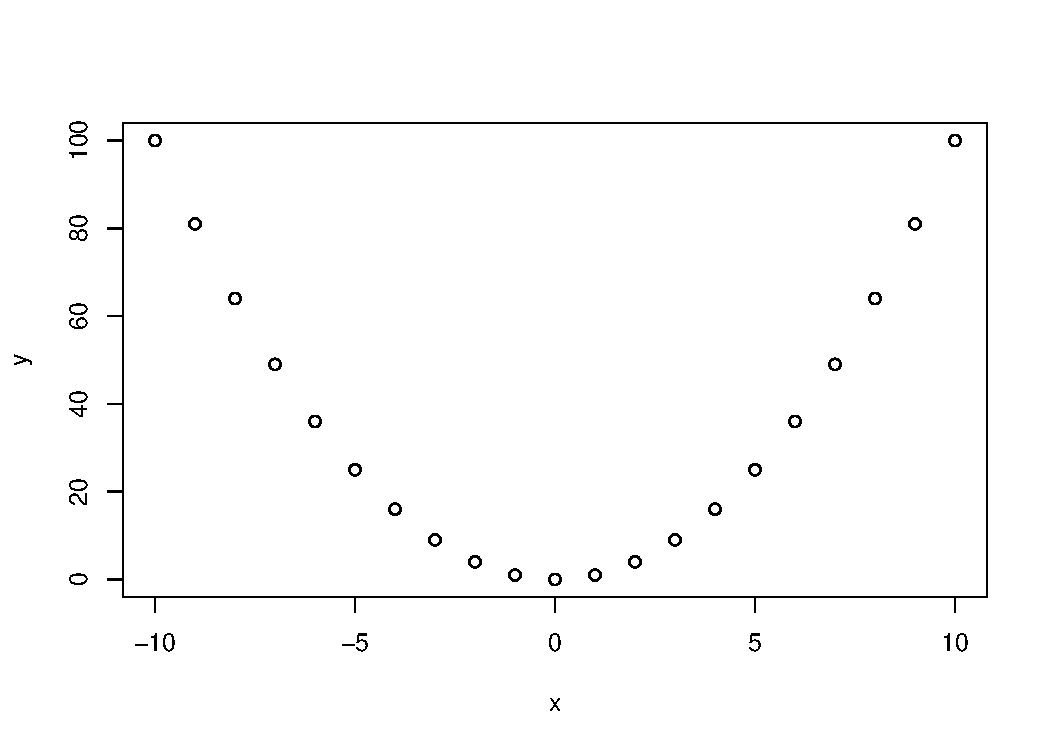
\includegraphics[width=4in]{plots/01.pdf} 
\end{figure}

To get a fast histogram we can do the following:

\begin{lstlisting}
> x <- rnorm(1000)
> hist(x, freq = FALSE)
\end{lstlisting}

\begin{figure}[h]
\centering
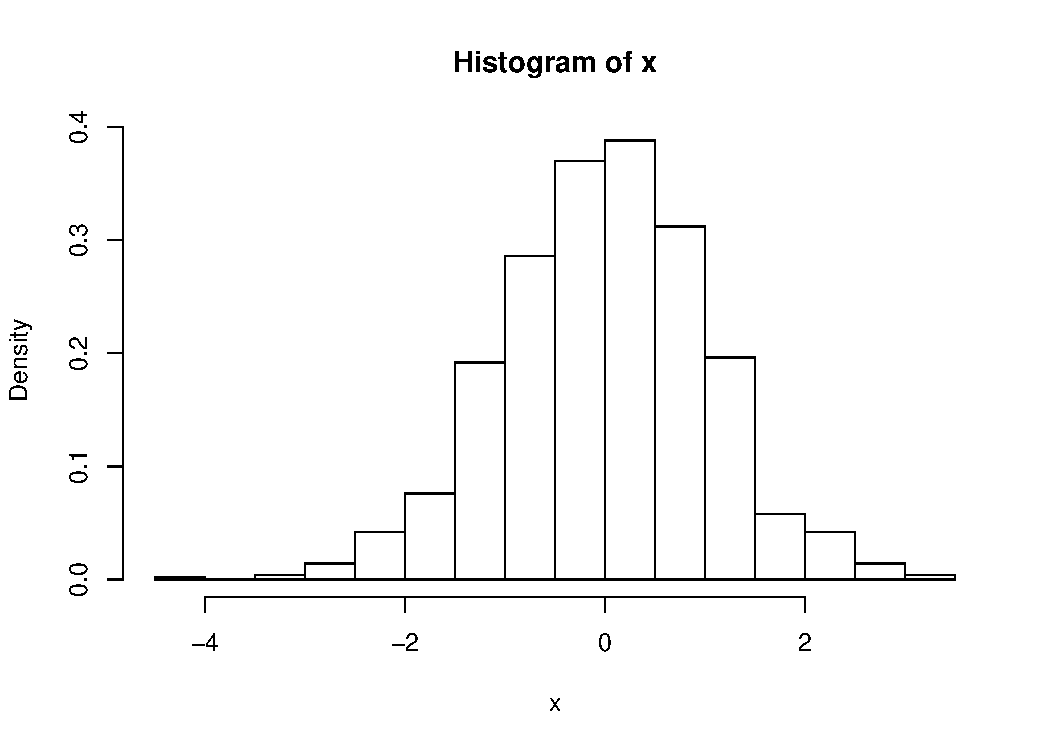
\includegraphics[width=4in]{plots/02.pdf} 
\end{figure}

\subsection{Scatterplots}

Let's start using \texttt{ggplot}. We're going to use a data set that is part of the \texttt{ggplot2} package. The data set \texttt{midwest} includes demographic information for counties in the Midwest.

\begin{lstlisting}
> library(ggplot2)
> data(midwest)

> colnames(midwest)
 [1] "PID"                  "county"               "state"               
 [4] "area"                 "poptotal"             "popdensity"          
 [7] "popwhite"             "popblack"             "popamerindian"       
[10] "popasian"             "popother"             "percwhite"           
[13] "percblack"            "percamerindan"        "percasian"           
[16] "percother"            "popadults"            "perchsd"             
[19] "percollege"           "percprof"             "poppovertyknown"     
[22] "percpovertyknown"     "percbelowpoverty"     "percchildbelowpovert"
[25] "percadultpoverty"     "percelderlypoverty"   "inmetro"             
[28] "category"   
\end{lstlisting}

\texttt{ggplot} relies on layers which are connected with the `+' sign. The first layer is created using the \texttt{ggplot} command on a data frame.

\begin{lstlisting}
> plot1 <- ggplot(midwest)
> plot1  # it's blank
\end{lstlisting}

To actually plot something we need to add another layer.

\begin{lstlisting}
# plot percentage of people with college degree vs percentage living below the poverty level
> plot1 <- ggplot(midwest) + 
+             geom_point(aes(x = percollege, y = percbelowpoverty))
> plot1
\end{lstlisting}

\begin{figure}[h]
\centering
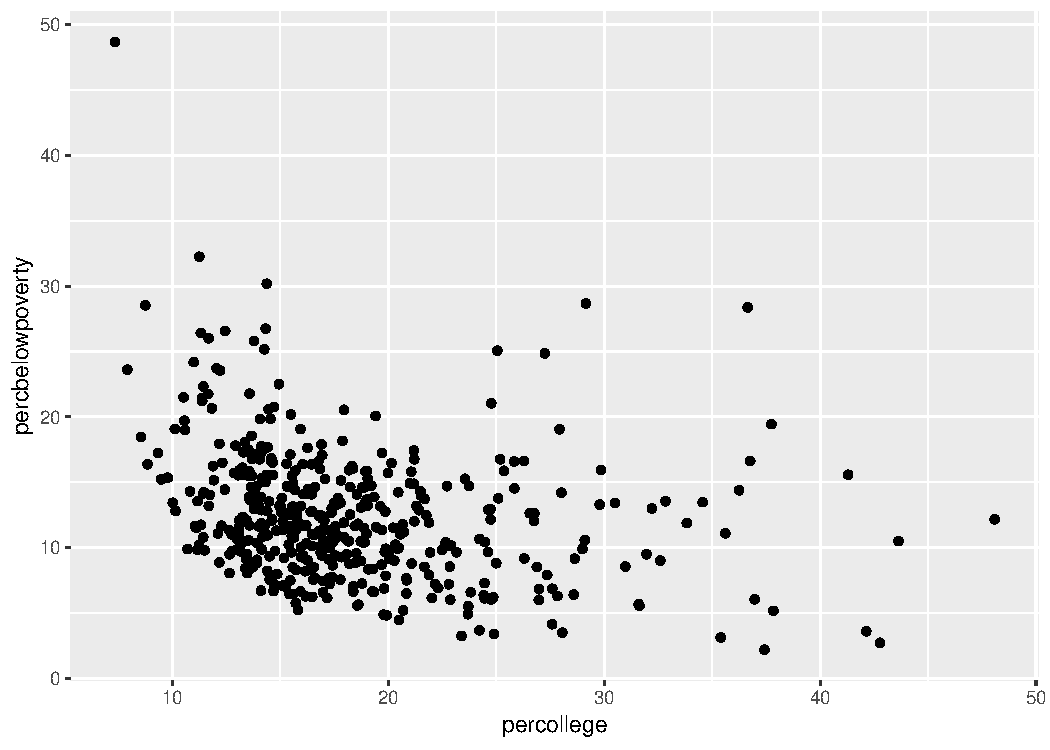
\includegraphics[width=4in]{plots/03.pdf} 
\end{figure}

Once a plot is created, it is pretty straight-forward to make changes to it. Let's say we want to add a title and change the axis labels.

\begin{lstlisting}
> plot1 <- plot1 +   # take plot1 and add
+            xlab("Percentage of people with college degree") +
+            ylab("Percentage of people below poverty line") +
+            ggtitle("College degrees and poverty")
> plot1
\end{lstlisting}

\begin{figure}[h]
\centering
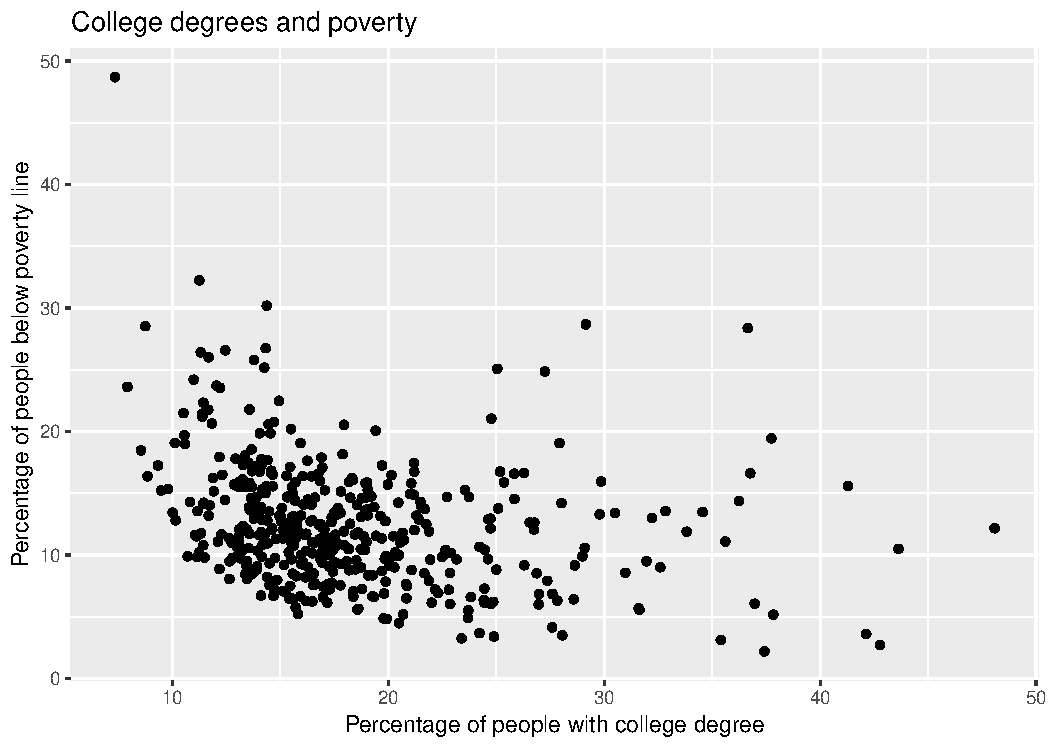
\includegraphics[width=4in]{plots/04.pdf} 
\end{figure}

We can add color by including a factor variable. In this case, let's color the observation by states.

\begin{lstlisting}
> midwest$state <- factor(midwest$state)  # needs to be a factor
> plot1 <- ggplot(midwest) +
+            geom_point(aes(x = percollege, y = percbelowpoverty, color = state)) +
+            xlab("Percentage of people with college degree") +
+            ylab("Percentage of people below poverty line") +
+            ggtitle("College degrees and poverty")
> plot1
\end{lstlisting}

\begin{figure}[h]
\centering
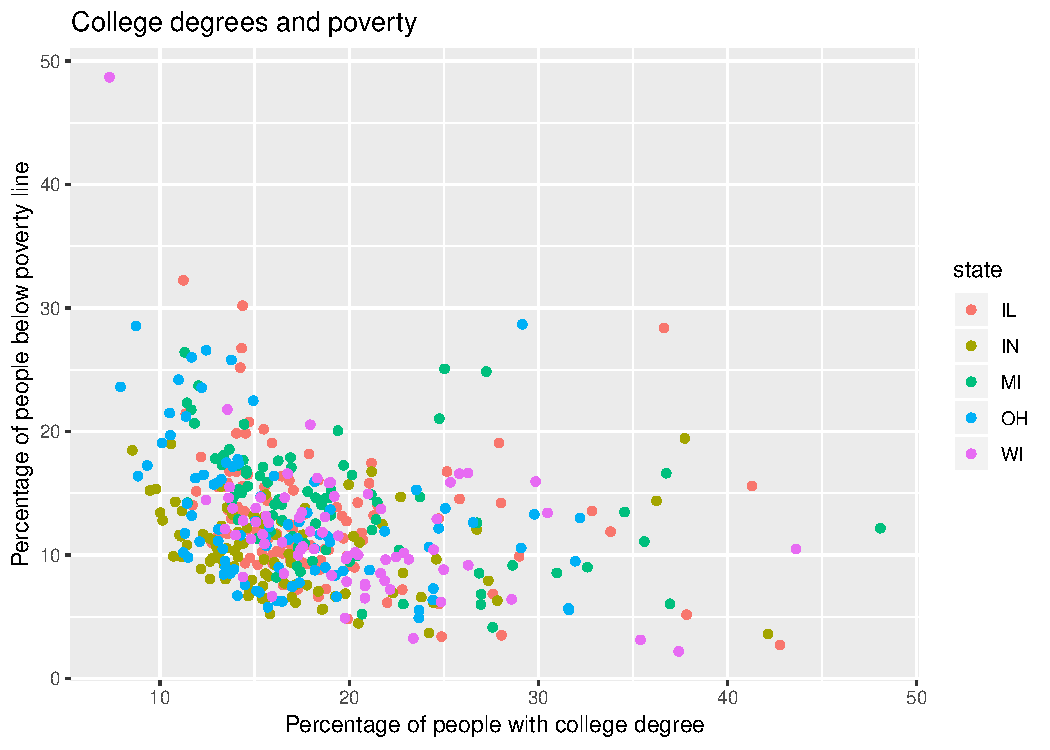
\includegraphics[width=4in]{plots/05.pdf} 
\end{figure}

Alternatively, we can also adjust the color, shape, and size of all points if we do so within \texttt{geom\_point} but outside \texttt{aes}.

\begin{lstlisting}
> plot1 <- ggplot(midwest) +
+            geom_point(aes(x = percollege, y = percbelowpoverty), col = "steelblue") +            
+            xlab("Percentage of people with college degree") +
+            ylab("Percentage of people below poverty line") +
+            ggtitle("College degrees and poverty")
> plot1
\end{lstlisting}

\begin{figure}[h]
\centering
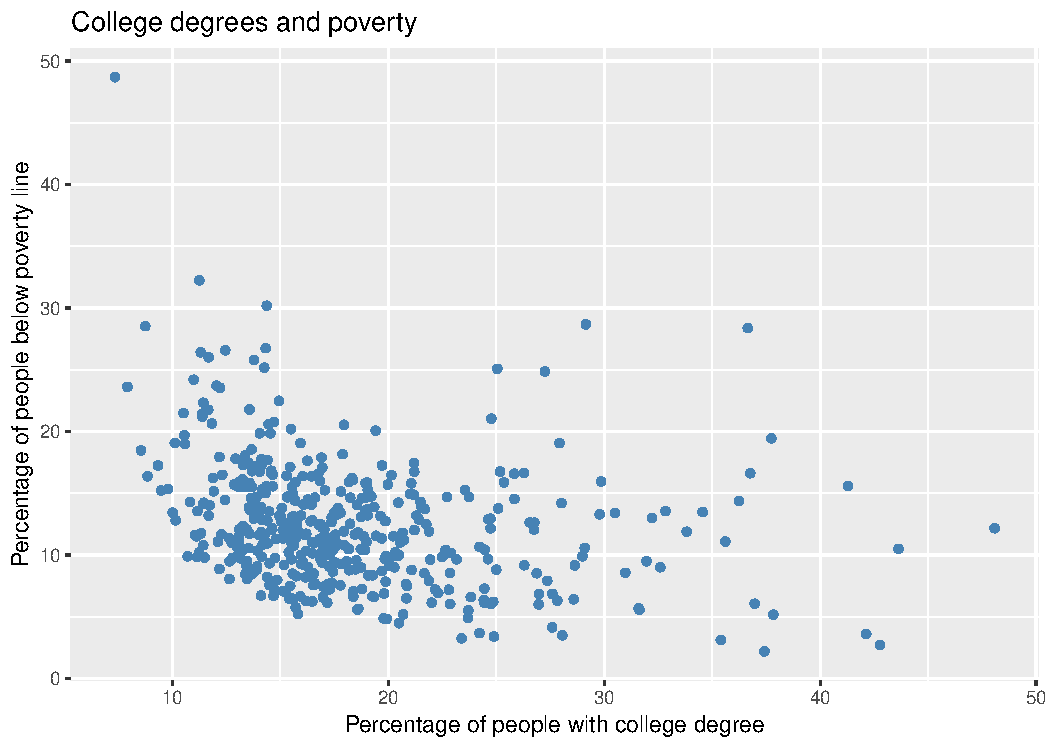
\includegraphics[width=4in]{plots/06.pdf} 
\end{figure}

Other things we can change are the background theme and the font size.

\begin{lstlisting}
> plot1 + 
+   theme_bw(20)
\end{lstlisting}

\begin{figure}[h]
\centering
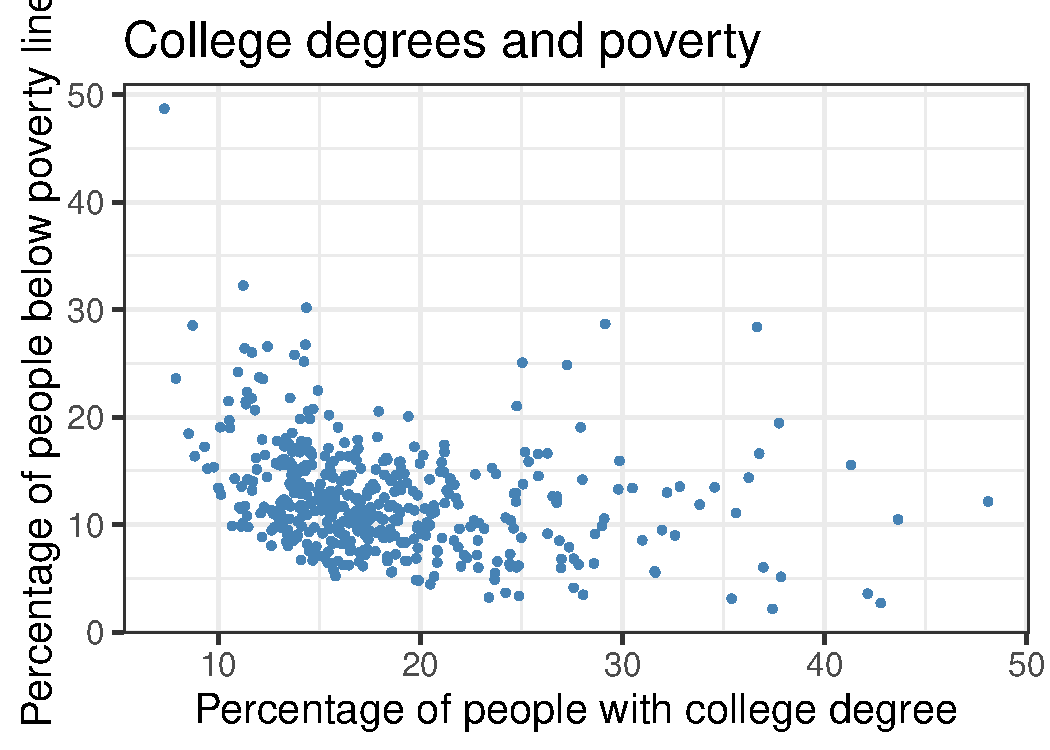
\includegraphics[width=4in]{plots/07.pdf} 
\end{figure}

\subsection{Adding features}

It is easy to add more features to a \texttt{ggplot}, just like we did with adding a title and axis labels. Now we'll add a best fit line, an arbitrary line, and a rug plot.

\begin{lstlisting}
> plot2 <- ggplot(midwest, aes(x = percollege, y = percbelowpoverty)) +
+            geom_point() +            
+            geom_smooth(method = "lm", size = 1) + # best fit line
+            geom_abline(intercept = 2, slope = 1
+                        , color = "red", size = 2) +
+            geom_rug(sides = "b")  # bottom rug plot
> plot2
\end{lstlisting}

\begin{figure}[h!]
\centering
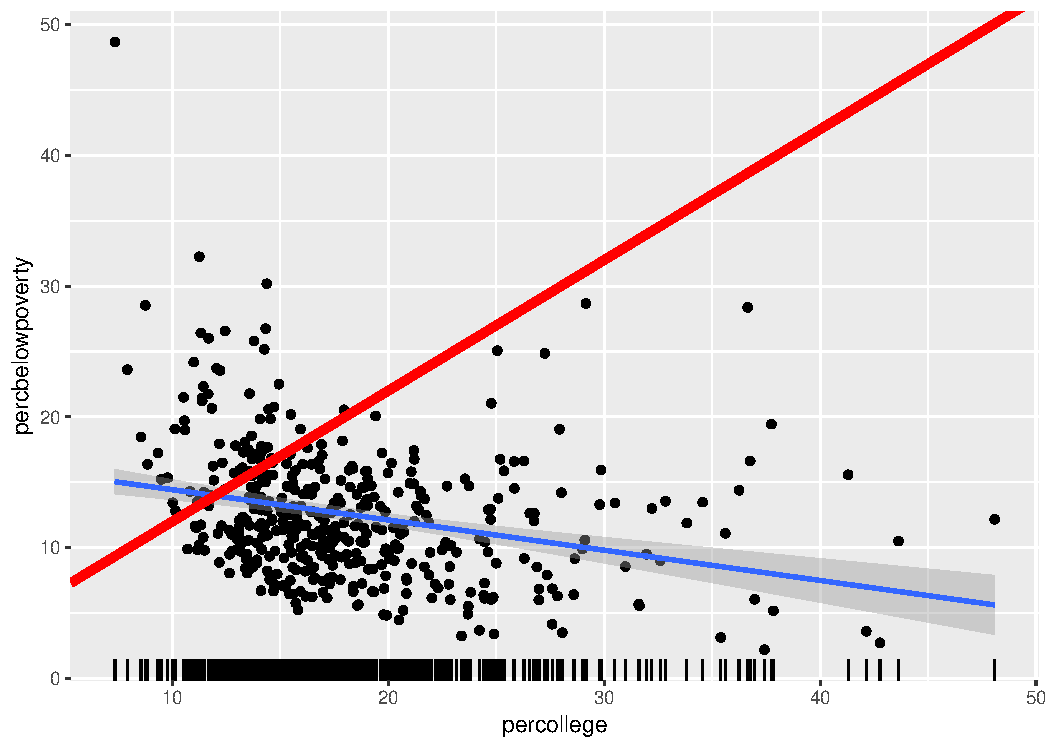
\includegraphics[width=4in]{plots/08.pdf} 
\end{figure}

\subsection{Other plots}

\subsubsection*{Histogram}

\begin{lstlisting}
> plot3 <- ggplot(midwest, aes(x = percollege)) +  # only need x for histogram
+             geom_histogram(binwidth = 1)
> plot3
\end{lstlisting}

\begin{figure}[h]
\centering
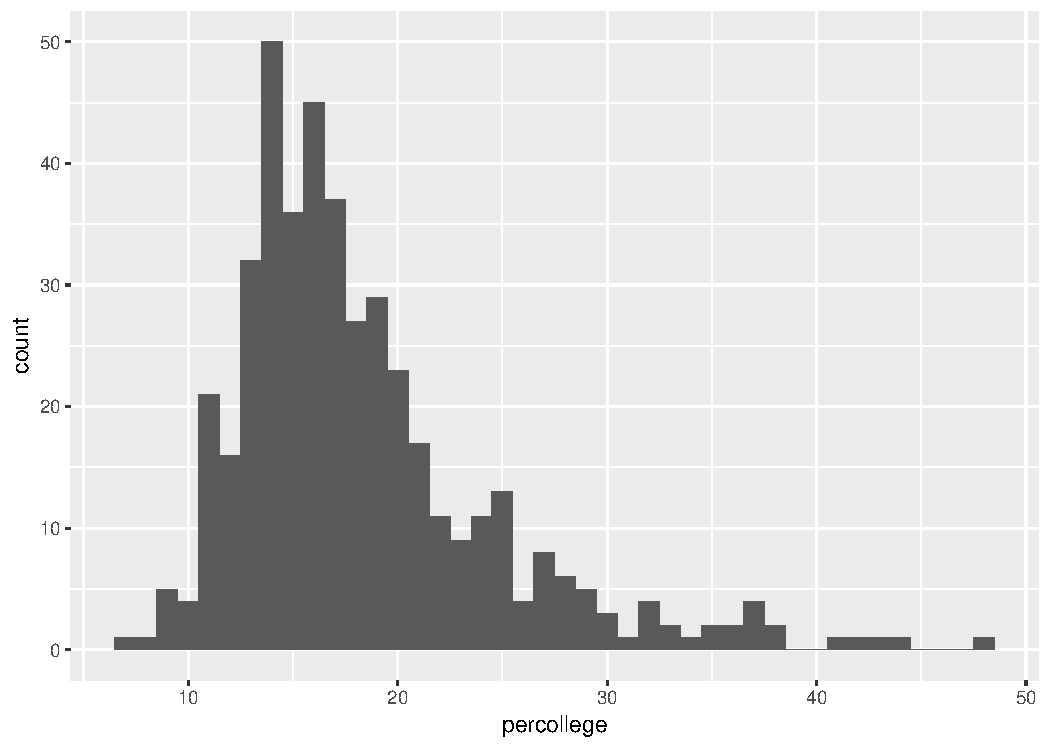
\includegraphics[width=4in]{plots/09.pdf} 
\end{figure}

I specified the bin width here, if you do not do that \R will choose something automatically. Let's change the colors and the axis labels.

\begin{lstlisting}
> plot3 <- plot3 +
+           geom_histogram(binwidth = 1
+                          , color = "black"  # outline
+                          , fill = "white")+ # inside
+           ylab("Count") +
+           xlab("Percentage of people with college degree")
> plot3
\end{lstlisting}

\begin{figure}[h]
\centering
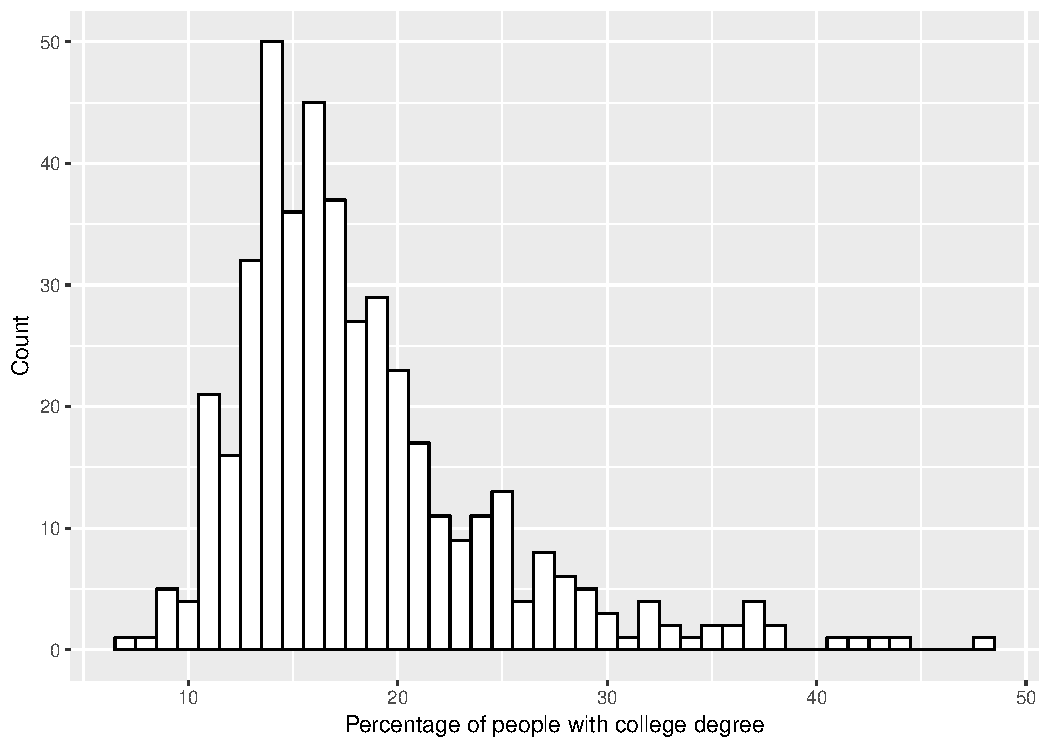
\includegraphics[width=4in]{plots/10.pdf} 
\end{figure}

\subsubsection*{Density}

A density plot is a smoothed version of the histogram for continuous data.

\begin{lstlisting}
> plot4 <- ggplot(midwest, aes(x = percollege)) + 
+             geom_density() +
+             ylab("Density") +
+             xlab("Percentage of people with college degree") +
+             ggtitle("Basic density")
> plot4
\end{lstlisting}

\begin{figure}[h]
\centering
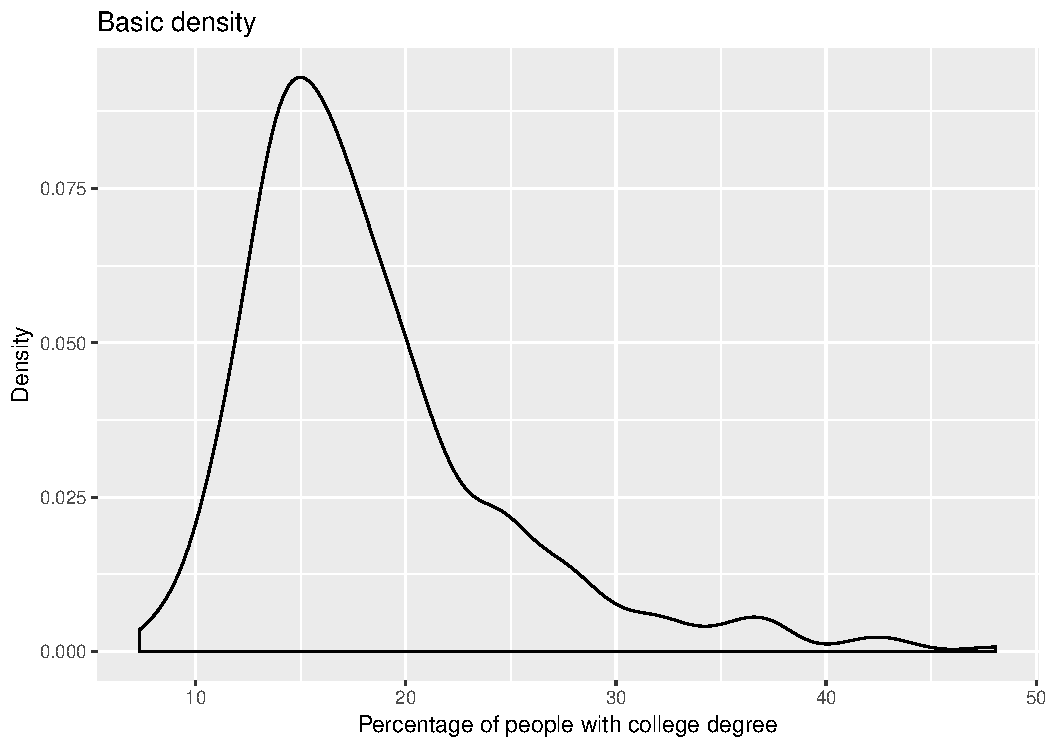
\includegraphics[width=4in]{plots/11.pdf} 
\end{figure}

We can check whether it matches the histogram by overlapping the two.

\begin{lstlisting}
> plot4 <-  ggplot(midwest, aes(x = percollege)) +
+           geom_histogram(aes(y =..density..)
+                          , binwidth = 1
+                          , color = "black"
+                          , fill = "white") +
+           geom_density(alpha = .2, fill = "#FF6666") +
+           ylab("Density") +
+           xlab("Percentage of people with college degree") +
+           ggtitle("Density + Histogram")
> plot4
\end{lstlisting}

\begin{figure}[h]
\centering
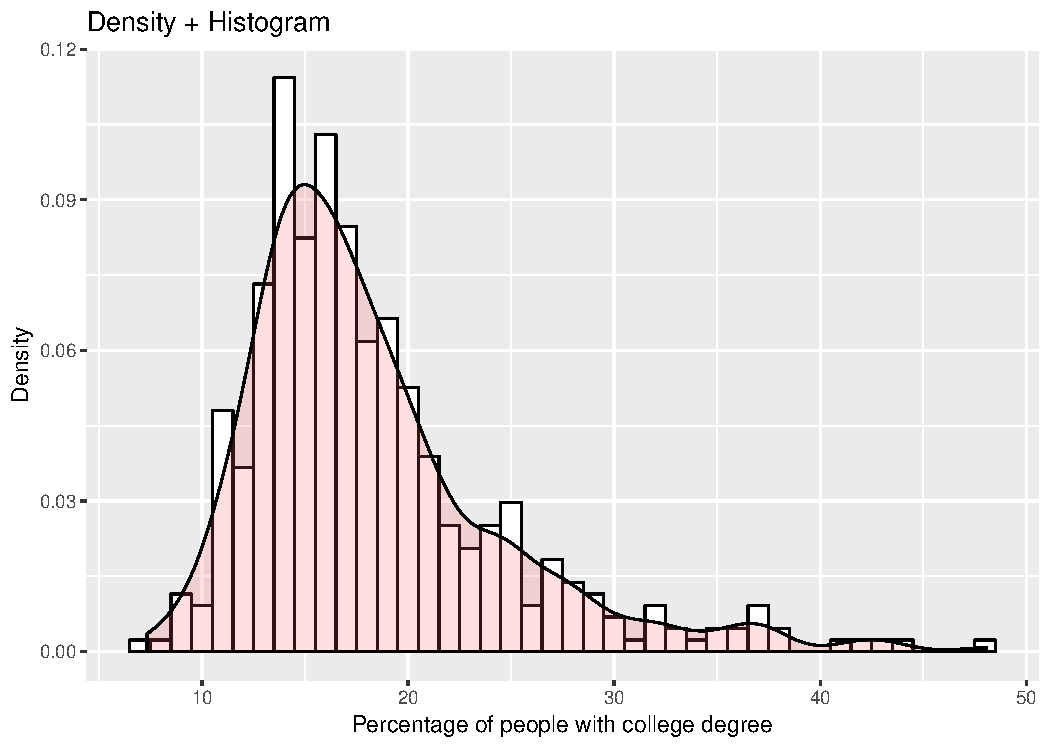
\includegraphics[width=4in]{plots/12.pdf} 
\end{figure}

\subsection{Saving plots}

To save individual plots you can do the following

\begin{lstlisting}
> ggsave(plot4, file = "plot4.pdf", height = 4, width = 6)  # saves into your working directory
\end{lstlisting}


	

\newpage
\section{Statistical analyses}
\subsection{Ordinary least squares}

We're going to use the same dataset by Fearon and Laitin again.

\begin{lstlisting}
library(foreign)
fl <- read.dta("fearonlaitin2003.dta")  # change to path on your computer
\end{lstlisting}

OLS in \R is done with the \texttt{lm} command. It takes formulas in the following form: \verb|Y ~ X1 + X2...|, where \texttt{Y} is the dependent variable and the \texttt{X}s are the independent variables. The tilde is used to separate them. We can also include \texttt{-1} if we want to drop the constant term. Check out \texttt{help(lm)} to see additional options and arguments.

\begin{lstlisting}
> # basic OLS
> model1 <- lm(onset ~ ethfrac
+              , data = fl)

# run only on former British colonies (variable: colbrit)
> model2 <- lm(onset ~ ethfrac
+              , data = fl
+              , subset = colbrit == 1)
\end{lstlisting}

We can make most adjustments to the formula with \texttt{I()} such as squared variables. We can also include interaction term or transform variables.

\begin{lstlisting}
# includes population and population squared
> model3 <- lm(onset ~ ethfrac + pop + I(pop^2)
+              , data = fl)

# interaction between ethnic fractionalization and population
> model4 <- lm(onset ~ ethfrac * pop
+              , data = fl)
\end{lstlisting}

\subsection{Extracting model information}

The value of \texttt{lm()} is a fitted model object; technically it is a list of results of class \texttt{"lm"}. Information can be extracted using different functions such as \texttt{summary}, \texttt{family}, \texttt{predict}, \texttt{residuals}, \texttt{coef}, and others. \texttt{summary()} is the most common command since it give you a very comprehensive summary of the results of regression analysis. Let's have a look at our last regression model, \texttt{model4}.

\begin{lstlisting}
> summary(model4)

Call:
lm(formula = onset ~ ethfrac * pop, data = fl)

Residuals:
    Min      1Q  Median      3Q     Max 
-0.1068 -0.0215 -0.0156 -0.0113  3.9667 

Coefficients:
             Estimate Std. Error t value Pr(>|t|)   
(Intercept) 8.459e-03  3.017e-03   2.804  0.00507 **
ethfrac     1.835e-02  6.361e-03   2.884  0.00393 **
pop         4.628e-08  2.479e-08   1.867  0.06192 . 
ethfrac:pop 4.235e-08  4.813e-08   0.880  0.37894   
---
Signif. codes:  0 ‘***’ 0.001 ‘**’ 0.01 ‘*’ 0.05 ‘.’ 0.1 ‘ ’ 1

Residual standard error: 0.138 on 6429 degrees of freedom
  (177 observations deleted due to missingness)
Multiple R-squared:  0.004104,	Adjusted R-squared:  0.003639 
F-statistic:  8.83 on 3 and 6429 DF,  p-value: 7.719e-06
\end{lstlisting}

We can also pull out information individually:

\begin{lstlisting}
> model4$coefficients
 (Intercept)      ethfrac          pop  ethfrac:pop 
8.459111e-03 1.834898e-02 4.628410e-08 4.234679e-08 

> head(model4$residuals) # residuals
          1           2           3           4           5           6 
-0.02366425 -0.02372362 -0.02377133 -0.02393177 -0.02409515 -0.02435831
 
> head(model4$fitted.values)  # predicted values
         1          2          3          4          5          6 
0.02366425 0.02372362 0.02377133 0.02393177 0.02409515 0.02435831 

> head(model4$model)  # data used to fit model
  onset   ethfrac    pop
1     0 0.3569501 140969
2     0 0.3569501 141936
3     0 0.3569501 142713
4     0 0.3569501 145326
5     0 0.3569501 147987
6     0 0.3569501 152273

> model4$call  # command used to create object
lm(formula = onset ~ ethfrac * pop, data = fl)

> vcov(model4)  # returns variance matrix of model
              (Intercept)       ethfrac           pop   ethfrac:pop
(Intercept)  9.104143e-06 -1.539275e-05 -2.088196e-11  3.474674e-11
ethfrac     -1.539275e-05  4.046649e-05  3.351982e-11 -9.699062e-11
pop         -2.088196e-11  3.351982e-11  6.144572e-16 -8.775865e-16
ethfrac:pop  3.474674e-11 -9.699062e-11 -8.775865e-16  2.316167e-15
\end{lstlisting}

\subsubsection*{Hypothesis testing}

The package \texttt{car} provides us with the useful command \texttt{linearHypothesis}.

\begin{lstlisting}
> # same as the basic t-test
> linearHypothesis(model4, c("ethfrac = 0"))
Linear hypothesis test

Hypothesis:
ethfrac = 0

Model 1: restricted model
Model 2: onset ~ ethfrac * pop

  Res.Df    RSS Df Sum of Sq      F   Pr(>F)   
1   6430 122.67                                
2   6429 122.51  1   0.15855 8.3201 0.003934 **
---
Signif. codes:  0 ‘***’ 0.001 ‘**’ 0.01 ‘*’ 0.05 ‘.’ 0.1 ‘ ’ 1

> # special test
> linearHypothesis(model4, c("ethfrac = 0.4"))
Linear hypothesis test

Hypothesis:
ethfrac = 0.4

Model 1: restricted model
Model 2: onset ~ ethfrac * pop

  Res.Df    RSS Df Sum of Sq      F    Pr(>F)    
1   6430 191.10                                  
2   6429 122.51  1    68.591 3599.5 < 2.2e-16 ***
---
Signif. codes:  0 ‘***’ 0.001 ‘**’ 0.01 ‘*’ 0.05 ‘.’ 0.1 ‘ ’ 1

> # test if they have the same coefficient
> linearHypothesis(model4, c("ethfrac = ethfrac:pop"))
Linear hypothesis test

Hypothesis:
ethfrac - ethfrac:pop = 0

Model 1: restricted model
Model 2: onset ~ ethfrac * pop

  Res.Df    RSS Df Sum of Sq    F   Pr(>F)   
1   6430 122.67                              
2   6429 122.51  1   0.15854 8.32 0.003934 **
---
Signif. codes:  0 ‘***’ 0.001 ‘**’ 0.01 ‘*’ 0.05 ‘.’ 0.1 ‘ ’ 1
\end{lstlisting}

\subsubsection*{Fixed effects and clustered errors}

One options to include fixed effects is by including dummy variables.

\begin{lstlisting}
> FE.model1 <- lm(onset ~ ethfrac + factor(ccode)
+                 , data = fl)
\end{lstlisting}

By introducing a dummy variable for every country in the dataset, you create a huge output. It's easier on the eyes to use the \texttt{plm} package instead. It suppresses the fixed effects in its output.

\begin{lstlisting}
> library(plm)
Loading required package: Formula
> FE.model2 <- plm(onset ~ ethfrac
+                  , model = "within"  # FE command
+                  , index = c("ccode", "year")  # panel variables
+                  , data = fl)

> summary(FE.model2)
Oneway (individual) effect Within Model

Call:
plm(formula = onset ~ ethfrac, data = fl, model = "within", index = c("ccode", 
    "year"))

Unbalanced Panel: n = 161, T = 7-55, N = 6610

Residuals:
    Min.  1st Qu.   Median  3rd Qu.     Max. 
-0.21272 -0.02500  0.00000  0.00000  3.91118 

Coefficients:
        Estimate Std. Error t-value  Pr(>|t|)    
ethfrac -0.37153    0.10575 -3.5133 0.0004456 ***
---
Signif. codes:  0 ‘***’ 0.001 ‘**’ 0.01 ‘*’ 0.05 ‘.’ 0.1 ‘ ’ 1

Total Sum of Squares:    119.69
Residual Sum of Squares: 119.47
R-Squared:      0.0019106
Adj. R-Squared: -0.023011
F-statistic: 12.3433 on 1 and 6448 DF, p-value: 0.00044562
\end{lstlisting}

You can get a random effects model by changing the \texttt{model} argument to \texttt{model = "random"}. You can also use \texttt{plm}'s built-in clustering functions.

\begin{lstlisting}
> # same as lm with clustering
> pool1 <- plm(onset ~ ethfrac
+                  , model = "pooling" 
+                  , index = c("ccode", "year") 
+                  , data = fl)

> # panel corrected standard errors
> pcse <- vcovBK(pool1, cluster = "time")
> coeftest(pool1, pcse)

t test of coefficients:

             Estimate Std. Error t value  Pr(>|t|)    
(Intercept) 0.0094397  0.0023773  3.9707 7.241e-05 ***
ethfrac     0.0202591  0.0064428  3.1445  0.001671 ** 
---
Signif. codes:  
0 ‘***’ 0.001 ‘**’ 0.01 ‘*’ 0.05 ‘.’ 0.1 ‘ ’ 1
\end{lstlisting}

We can do the same for fixed effects models.

\begin{lstlisting}
> # fixed effects model, standard errors clustered on country
> clust <- vcovBK(FE.model2, cluster = "group")  # can be either "group" or "time" or both
> coeftest(FE.model2, clust)

t test of coefficients:

         Estimate Std. Error t value  Pr(>|t|)    
ethfrac -0.371531   0.076281 -4.8706 1.139e-06 ***
---
Signif. codes:  
0 ‘***’ 0.001 ‘**’ 0.01 ‘*’ 0.05 ‘.’ 0.1 ‘ ’ 1

\end{lstlisting}

\subsection{Output into tables}

You might want to include the output of your regression models into a paper. We will cover two packages that let you export tables into \LaTeX (or HTML).

\subsubsection*{\texttt{xtable}}

\begin{lstlisting}
> library(xtable)
> xtable(model1)
% latex table generated in R 3.5.0 by xtable 1.8-2 package
% Wed Sep 26 17:11:06 2018
\begin{table}[ht]
\centering
\begin{tabular}{rrrrr}
  \hline
 & Estimate & Std. Error & t value & Pr($>$$|$t$|$) \\ 
  \hline
(Intercept) & 0.0094 & 0.0028 & 3.34 & 0.0009 \\ 
  ethfrac & 0.0203 & 0.0059 & 3.43 & 0.0006 \\ 
   \hline
\end{tabular}
\end{table}
\end{lstlisting}

In \LaTeX, this looks like this:

% latex table generated in R 3.5.0 by xtable 1.8-2 package
% Wed Sep 26 17:11:06 2018
\begin{table}[h]
\centering
\begin{tabular}{rrrrr}
  \hline
 & Estimate & Std. Error & t value & Pr($>|t|$) \\ 
  \hline
(Intercept) & 0.0094 & 0.0028 & 3.34 & 0.0009 \\ 
  ethfrac & 0.0203 & 0.0059 & 3.43 & 0.0006 \\ 
   \hline
\end{tabular}
\end{table}

\subsubsection*{\texttt{stargazer}}

This package is useful when we want to display models side by side. Unlike \texttt{xtable} it works on nearly every canned model directly.

\begin{lstlisting}
> library(stargazer)

> stargazer(model2, model3, FE.model2
+           , title = "Trying out Stargazer"
+           , label = "tab:stargazer"
+           , covariate.labels = c("Ethnic Frac."
+                                 , "Population"
+                                 , "Ethnic Frac. * Population")
+           , dep.var.labels = "Onset"
+           , digits = 2
+           , style = "AJPS")  # choose a journal to emulate

% Table created by stargazer v.5.2.2 by Marek Hlavac, Harvard University. E-mail: hlavac at fas.harvard.edu
% Date and time: Thu, Sep 27, 2018 - 04:59:11 PM
\begin{table}[!htbp] \centering 
  \caption{Trying out Stargazer} 
  \label{tab:stargazer} 
\begin{tabular}{@{\extracolsep{5pt}}lccc} 
\\[-1.8ex]\hline \\[-1.8ex] 
\\[-1.8ex] & \multicolumn{3}{c}{\textbf{Onset}} \\ 
\\[-1.8ex] & \multicolumn{2}{c}{\textbf{OLS}} & \textbf{panel} \\ 
 & \multicolumn{2}{c}{\textbf{}} & \textbf{linear} \\ 
\\[-1.8ex] & \textbf{Model 1} & \textbf{Model 2} & \textbf{Model 3}\\ 
\hline \\[-1.8ex] 
 Ethnic Frac. & 0.01 & 0.02$^{***}$ & $-$0.37$^{***}$ \\ 
  & (0.01) & (0.01) & (0.11) \\ 
  Population &  & 0.0000$^{***}$ &  \\ 
  &  & (0.0000) &  \\ 
  Ethnic Frac. * Population &  & $-$0.00$^{**}$ &  \\ 
  &  & (0.00) &  \\ 
  Constant & 0.01$^{**}$ & 0.01$^{**}$ &  \\ 
  & (0.01) & (0.003) &  \\ 
 N & 1896 & 6433 & 6610 \\ 
R-squared & 0.0002 & 0.005 & 0.002 \\ 
Adj. R-squared & $-$0.0003 & 0.004 & $-$0.02 \\ 
Residual Std. Error & 0.13 (df = 1894) & 0.14 (df = 6429) &  \\ 
F Statistic & 0.34 (df = 1; 1894) & 10.16$^{***}$ (df = 3; 6429) & 12.34$^{***}$ (df = 1; 6448) \\ 
\hline \\[-1.8ex] 
\multicolumn{4}{l}{$^{***}$p $<$ .01; $^{**}$p $<$ .05; $^{*}$p $<$ .1} \\ 
\end{tabular} 
\end{table} 
\end{lstlisting}

Using the \texttt{out} option, you can also directly save this to a \texttt{.tex} file. The table looks as follows:

% Table created by stargazer v.5.2.2 by Marek Hlavac, Harvard University. E-mail: hlavac at fas.harvard.edu
% Date and time: Thu, Sep 27, 2018 - 04:59:11 PM
\begin{table}[!h] \centering 
  \caption{Trying out Stargazer} 
  \label{tab:stargazer} 
\begin{tabular}{@{\extracolsep{5pt}}lccc} 
\\[-1.8ex]\hline \\[-1.8ex] 
\\[-1.8ex] & \multicolumn{3}{c}{\textbf{Onset}} \\ 
\\[-1.8ex] & \multicolumn{2}{c}{\textbf{OLS}} & \textbf{panel} \\ 
 & \multicolumn{2}{c}{\textbf{}} & \textbf{linear} \\ 
\\[-1.8ex] & \textbf{Model 1} & \textbf{Model 2} & \textbf{Model 3}\\ 
\hline \\[-1.8ex] 
 Ethnic Frac. & 0.01 & 0.02$^{***}$ & $-$0.37$^{***}$ \\ 
  & (0.01) & (0.01) & (0.11) \\ 
  Population &  & 0.0000$^{***}$ &  \\ 
  &  & (0.0000) &  \\ 
  Ethnic Frac. * Population &  & $-$0.00$^{**}$ &  \\ 
  &  & (0.00) &  \\ 
  Constant & 0.01$^{**}$ & 0.01$^{**}$ &  \\ 
  & (0.01) & (0.003) &  \\ 
 N & 1896 & 6433 & 6610 \\ 
R-squared & 0.0002 & 0.005 & 0.002 \\ 
Adj. R-squared & $-$0.0003 & 0.004 & $-$0.02 \\ 
Residual Std. Error & 0.13 (df = 1894) & 0.14 (df = 6429) &  \\ 
F Statistic & 0.34 (df = 1; 1894) & 10.16$^{***}$ (df = 3; 6429) & 12.34$^{***}$ (df = 1; 6448) \\ 
\hline \\[-1.8ex] 
\multicolumn{4}{l}{$^{***}$p $<$ .01; $^{**}$p $<$ .05; $^{*}$p $<$ .1} \\ 
\end{tabular} 
\end{table} 

\begin{lstlisting}

\end{lstlisting}

\subsection{Plotting results} 

\newpage
\section{Best practices for writing \R code}
\R code, just like any other code, is a form of language. While there is no official ``right'' way to write \R code, you should pay attention to the way you are writing it. A major reason for that is that your code is likely to be read by others such as coauthors or people you may ask for help troubleshooting it. Following some common style rules can make understanding each other's code much easier. It will also help yourself read your own code or troubleshoot it.

A lot of style recommendations for \R code are based on Google's \href{https://google.github.io/styleguide/Rguide.xml}{style guide}. It's a useful starting point and a good resource. However, any kind of rules you adopt must work for you and are always subjective. In the following, I list some of the most widely accepted guidelines that I also agree with.

\subsection{Naming conventions}

For naming objects, there is the trade-off between being descriptive and being concise. Names should be meaningful in order to tell the reader what it contains but not long enough to get tedious and unnecessary. For example \texttt{sleep\_students} might be preferred to \texttt{hours\_students\_sleep\_at\_night}.

Besides the actual names, people have different conventions of capitalization and expressing spaces. For example,

{\parindent40pt % disables indentation for all the text between { and }
	{\small \texttt{maximization\_function}}
	
	{\small \texttt{maximization.function}}
	
	{\small \texttt{MaximizationFunction}}
	
	{\small \texttt{maximizationfunction}}
}

Choose one of the conventions and stick to it. Some people choose different ones for different types of objects. Avoid names that are reserved by \R commands and other important words that \R uses such as \texttt{T}, \texttt{F}, \texttt{else}, etc. 

\subsection{File organization}

\subsection{Syntax}

\subsection{Additional conventions}

%\bibliography{library}

\end{document}
